\documentclass{lecturesimple}

\newcommand{\DateOfShow}{2021-08-25}
\newcommand{\Startdag}{måndag}
\newcommand{\KursStartTidDod}{mån kl 10:15 Online}
\newcommand{\KursStartTidPgk}{mån kl 15:15 Hybrid (E:A+Online)}

\title{Hur plugga programmering?}
\author{cs.lth.se/bjorn-regnell}
\institute{}
\date{\DateOfShow}

\begin{document}

\frame{\titlepage}

% \begin{Slide}{Mål}
%   \begin{itemize}
%     \item Ge tips
%     \item Inspirera
%     \item Svara på frågor
%   \end{itemize}
%   % \vspace{3em}
%   % \footnotesize Källkoden för denna presentation:
%   % \\{\tiny\url{https://github.com/lunduniversity/introprog/blob/master/slides/info-week00-online.tex}}
% \end{Slide}

\begin{Slide}{Tips för framgång i programmeringsstudier}
  \begin{itemize}
    \item Motivation att gå på djupet
    \item Hårt arbete
    \item Effektiv studieteknik
    \item Uppmuntrande socialt sammanhang
  \end{itemize}  
\end{Slide}

%\SlideImg{Stor spridning i förkunskaper på D\\(enkätsvar 2015)}{../img/survey-2015}

\SlideImg{Stor spridning i förkunskaper}{../img/survey-2021}

\begin{Slide}{Planeten Jordens 2 största utmaningar?}
  \begin{itemize}
    \item Klimatet
    \item Digitaliseringen 
  \end{itemize}
\end{Slide}

\begin{Slide}{Digitaliseringens 2 största utmaningar?}
  \begin{itemize}
    \item Komplexitet
    \item Kompetensbrist 
  \end{itemize}  
\end{Slide}

\SlideImg{Välutbildade inom IT är oerhört eftertraktade}{../img/kompetensbrist}


\begin{Slide}{Digitaliseringens 2 största risker?}
  \begin{itemize}
    \item Hotet mot demokratin
    \item Oacceptabla klyftor
  \end{itemize}  
\end{Slide}

\begin{Slide}{Dina 2 största utmaningar som blivande ingenjör?}
  \begin{itemize}
    \item Ständigt lära ny teknik genom hela livet 
    \item Kontinuerligt uppgradera din studieteknik
  \end{itemize}  
\end{Slide}


{
  \setbeamercolor{background canvas}{bg=black}
  \frame{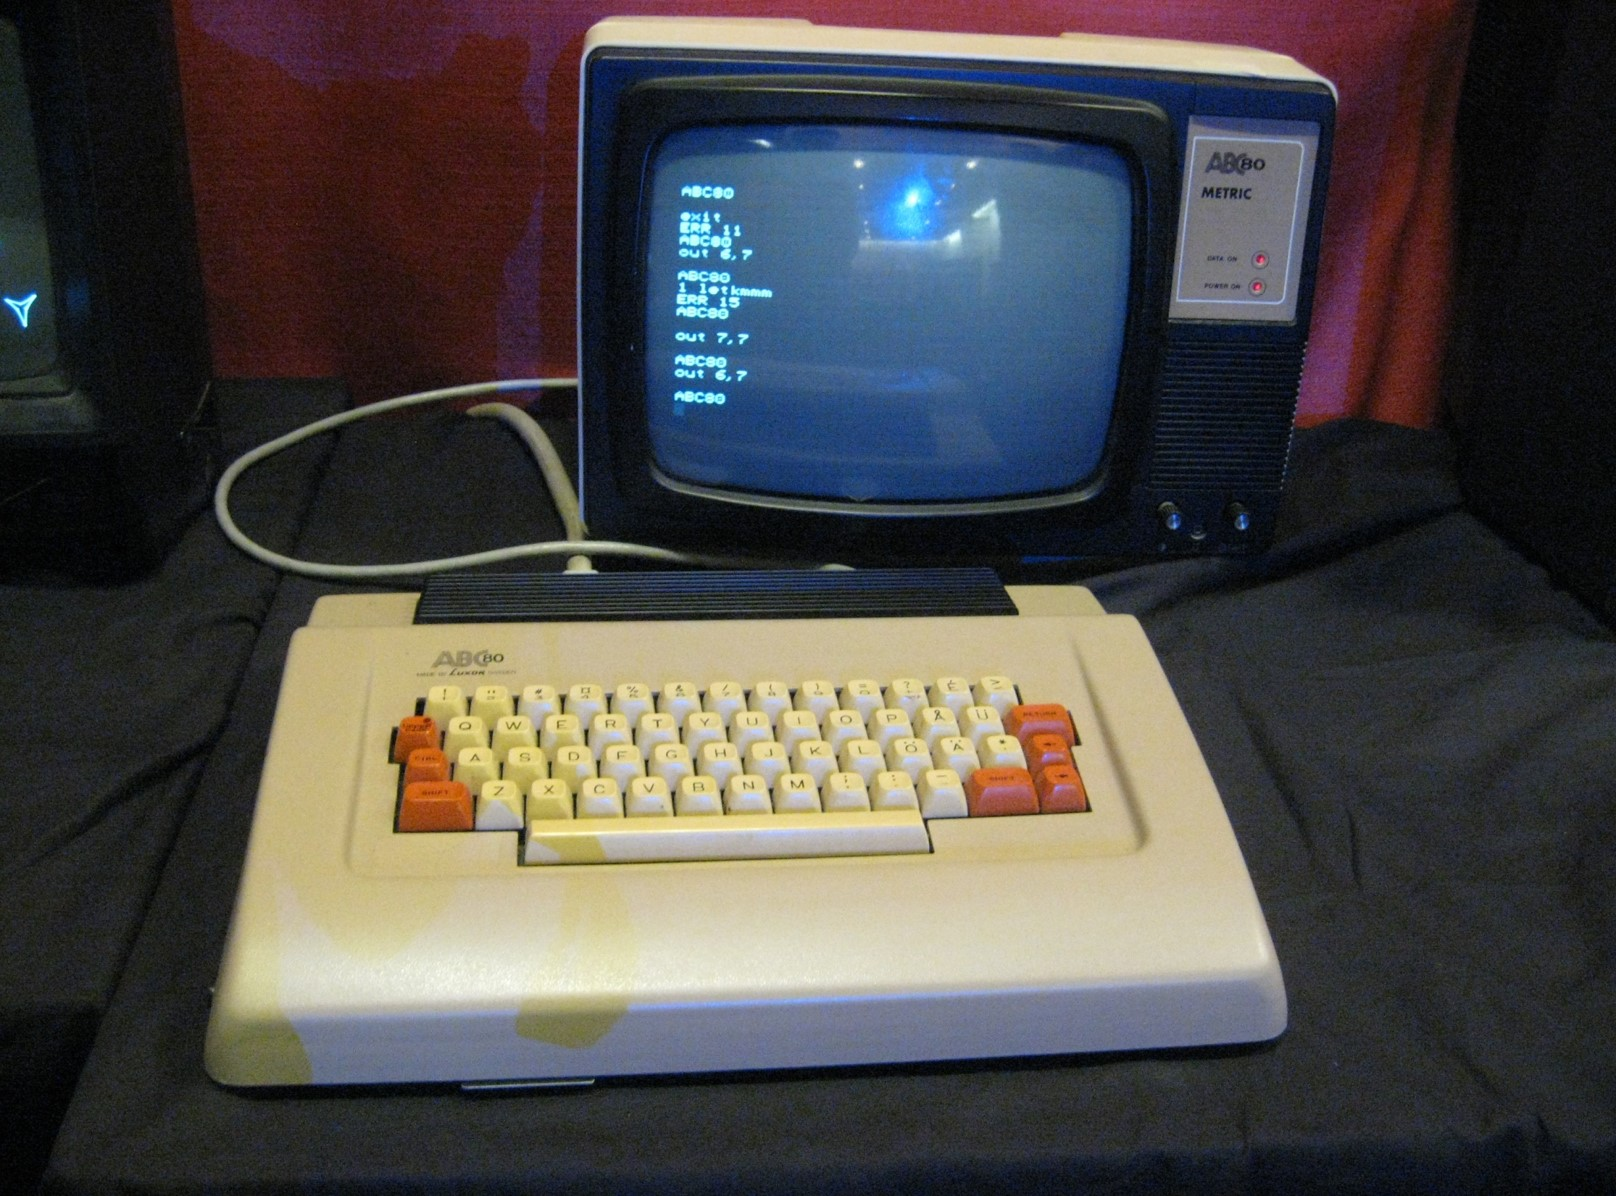
\includegraphics[width=1.0\textwidth]{../img/abc80}}
}

\begin{frame}\frametitle{Hårdvara 1986: IBM 3090, 69MHz, 128MB RAM}
\begin{center}
     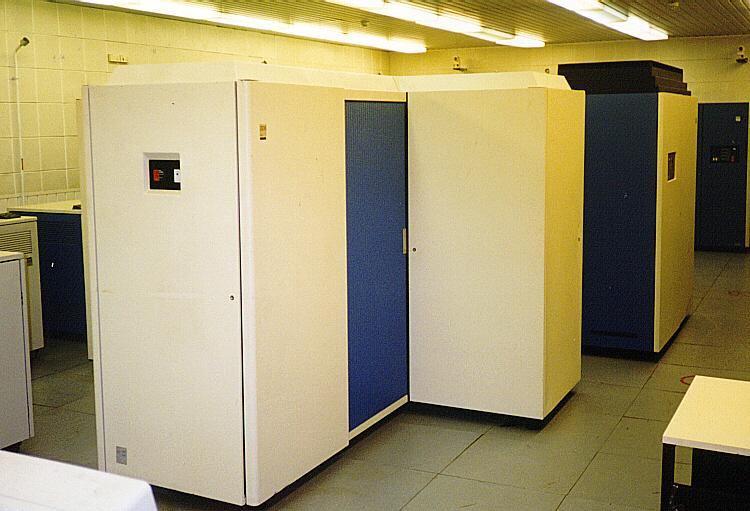
\includegraphics[width=1.0\textwidth]{../img/ibm3090.jpg}
%     % http://hampage.hu/oldiron/e_ibms.html
  
    {\fontsize{5}{5}\selectfont\color{gray}
    Foto: hampage.hu/oldiron
  }
\end{center}
\end{frame}
  
\begin{frame}\frametitle{Hårdvara 2014: Facebooks serverhall i Luleå, \\ 28000 kvm, 1 terrawatttimme per år}
  \begin{center}
    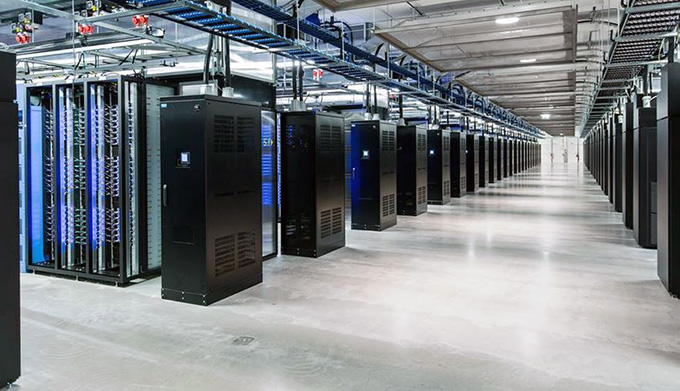
\includegraphics[width=1.05\textwidth]{../img/lulea-datacenter.jpg}
    % https://nyadagbladet.se/wp-content/uploads/2013/06/lulea-datacenter.jpg
    % http://gamla.hbl.fi/nyheter/2013-07-06/471016/facebook-placerade-serverhallar-i-lulea
  
    {\fontsize{5}{5}\selectfont\color{gray}
  Foto: Facebook
  }
  \end{center}
\end{frame}

\begin{Slide}{Kurskombo startar \Startdag}
  Grunden för kommande kurser: \vspace{2em}
  \begin{itemize}
    \item \Alert{Programmering, grundkurs} (pgk), 7.5 hp, 16 veckor
    \begin{itemize}
      \item[]
      \item[]
    \end{itemize}
    \item \Alert{Datorer och datoranvändning} (dod), 3 hp, 3 veckor
    \begin{itemize}
      \item[] 
      \item[] 
    \end{itemize}
  \end{itemize}
\end{Slide}

\begin{Slide}{Kurskombo startar \Startdag}
  Grunden för kommande kurser: \vspace{2em}
  \begin{itemize}
    \item \Alert{Programmering, grundkurs} (pgk), 7.5 hp, 16 veckor
    \begin{itemize}
      \item Programmering \Emph{från början}
      \item Stora möjligheter till valfri \Emph{fördjupning}
    \end{itemize}
    \item \Alert{Datorer och datoranvändning} (dod), 3 hp, 3 veckor
    \begin{itemize}
      \item Inblick i hur datorer fungerar och verktygen vi använder
      \item För C-are ingår dod i digitaliseringskursen (EITA65)
    \end{itemize}
  \end{itemize}
\end{Slide}

% \begin{Slide}{Några pedagogiska angreppssätt}
%   \begin{itemize}
%     \item Fokus på förståelse av begrepp, språk som tankeverktyg 
%     \item Fokus på förståelse genom skapande och experimentlusta
%     \item Variationsmönster: 
%     \begin{itemize}
%       \item Kontrastera
%       \item Generalisera
%       \item Separera
%       \item Sammanföra
%     \end{itemize} 
%     \item Omfamna önskvärda svårigheter
%     \item Hög ambition och goda möjligheter till fördjupning
%   \end{itemize}
% \end{Slide}

\begin{Slide}{Vad ska du lära dig?}
  \begin{itemize}
    \item Tänka i abstraktioner
    \item Skapa kod
    \item Ett nytt språk -- verktyg för tanken (Scala)
  \end{itemize}
\end{Slide}

% \frame{\frametitle{Vad ska du lära dig?}
% %Att skapa koden som styr världen...
% %\includegraphics[width=1.2\textwidth, height=1.5cm]{img/code-wide}
% \begin{multicols}{2}
% \begin{itemize}\Size{9pt}
% \item \textbf{Programmering, grundkurs}
% \begin{itemize}\Size{8pt}
% \item Tänka i abstraktioner
% \item Använda datastrukturer
% \item Implementera algoritmer
% \item Brepp som lägger grunden för resten av din utbildning
% \item Språk: \Emph{Scala} (och lite Java)
% \end{itemize}
% \columnbreak
% \item \textbf{Datorer \& datoranvändning}
% \begin{itemize}\Size{8pt}
% \item Lågnivåprogrammering
% \item Datarepresentation
% \item Terminalkommando i Linux
% \item Skriva \& typsätta i \LaTeX
% \item Beräkningar i Matlab
% \end{itemize}
% \end{itemize}
% \end{multicols}
% }

%%%
\frame{\frametitle{Hur ska du lära dig?}
\begin{itemize}
\item Praktiskt eget arbete: Lära genom att göra!
\begin{itemize}
\item Övningar
\item Laborationer
\item Projekt
\end{itemize}
\item Använda nya begrepp och förstå dem på djupet
\item Samarbete med dina kursare
\end{itemize}
}

\begin{Slide}{Samarbetsgrupper}
  \begin{itemize}
    \item Du delas in i en samarbetsgrupp med förkunskapsspridning
    \item Odla din samarbetskultur
    \item Hjälpa att förstå men inte ge färdiga svar
  \end{itemize}
\end{Slide}

% %%
% \frame{\frametitle{Kurslitteratur}
% \footnotesize
% \begin{columns}
% \begin{column}{0.65\textwidth}
% {\Size{16pt}pgk:}
% \begin{itemize}
% \item 2 st kompendier 358+360 sidor \\ Säljs till självkostnadspris på institutionen. \\ Beställ bokpaket om du inte redan gjort det här \Alert{senast idag kl 12} för mängdrabatt: \url{http://cs.lth.se/pgk/bokpaket}
% \end{itemize}
% \vspace{1em}
% {\Size{16pt}dod:}
% \begin{itemize}
% \item Kursmaterial delas ut på första föreläsningen.
% \end{itemize}
% \end{column}
% \begin{column}{0.35\textwidth}
% \centering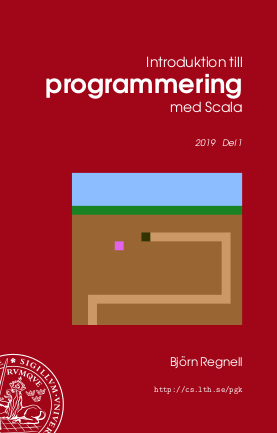
\includegraphics[width=0.99\textwidth]{../img/compendium-front-page-2019.png}
% \end{column}
% \end{columns}
% }


%%% AAAARGH -- version clash ? or something causing thins in Ubuntu 20.04 
%%%   but not in ubuntu 18.04:
%%%
  % ! Package pgfplots Error: Sorry, could not retrieve column 'år' from table 
  %'<inline_table>'. Please check spelling (or introduce name aliases)..

  % See the pgfplots package documentation for explanation.
  % Type  H <return>  for immediate help.
  %  ...                                              
                                                    
  % l.27 ...dplot table[x=år,y=nybörjare]{\dataSeq};


% \begin{Slide}{Andelen D-are som vid kursstart aldrig kodat}
% \pgfplotstableread[row sep=\\,col sep=&]{
%     år & nybörjare\\
%     2015 & 19  \\
%     2016 & 32  \\
%     2017 & 38  \\
%     2018 & 31  \\
%     2019 & 30  \\
%     2020 & 20  \\
%     }\dataSeq

% \begin{minipage}{0.65\textwidth}
% \hspace*{-0.65cm}%
% \begin{tikzpicture}[scale=0.9, every node/.style={scale=0.9}]
%     \begin{axis}[
%             ybar,
%             bar width=1.0cm,
%             symbolic x coords={2015,2016,2017,2018,2019,2020},
%             xtick=data,
%             nodes near coords,
%             nodes near coords align={vertical},
%             legend style={at={(0.5,1)},anchor=south,legend columns=-1,draw=none},
%             ymin=0,ymax=45,
%             ylabel={\%},
%             xlabel={År},
%         ]
%         \addplot table[x=år,y=nybörjare]{\dataSeq};
%         %\legend{nybörjare}
%     \end{axis}
% \end{tikzpicture}
% \end{minipage}%
% \begin{minipage}{0.3\textwidth}
% \begin{itemize}\SlideFontTiny
% \item[] År: antal enkätsvar D
% \item[] 2015: 102 st
% \item[] 2016: 104 st
% \item[] 2017: 114 st
% \item[] 2018: 123 st
% \item[] 2019: 125 st 
% \item[] 2020: 137 st 
% \end{itemize}
% \end{minipage}%
% \end{Slide}


%%%

% \frame[plain]{\frametitle{Grattis ni som beställt bokpaket!}
% Bokpaketet är \Emph{fantastiskt!}\\~\\
% \Alert{Om du vill efterbeställa gör det i Canvas}%\\ (Även om du svarar ''Nej'')
% }

% \frame[plain]{\frametitle{Förkunskapsenkät}

% Ditt svar på denna \Emph{förkunskapsenkät} används i planeringen:
% \url{http://cs.lth.se/pgk/introsurvey}\\
% \Alert{Om du inte fyllt i den gör det nu!}\\
% \vspace{1em}
% Enkäten innehåller dessa frågor och några till:
% \begin{itemize}
% \item Har du programmerat tidigare? \\
%          Ja \hspace{2.5cm} Nej
% \item Hur många program har du skrivit? \\
%          $<5$ \hspace{2.2cm} $5-20$ \hspace{2.5cm}  $>20$
% \item Hur stort var det största program du har skrivit?\\
%          $<50$ rader \hspace{1cm} $50 - 500$  rader \hspace{1cm}  $>500$ rader
% \end{itemize}
% \vspace{1em}
% }


\begin{Slide}{Bokpaket}
  \begin{itemize}
    %\item Det är 117 D-are, 4 W-are och 4 fristående som beställt kursmaterial. Grattis! :)
    \item Programstudenter får bokpaket mot uppvisande av Swish-transaktion via faddrar, enligt information i Canvas.
    \item De som missar fadderutdelningen samt W:are och fristående hämtar på cs expedition under expeditionstider mot uppvisande av Swish-transaktion enl information i Canvas.
    \item Efterbeställning möjlig via Canvas. De första 10 får lägre priset därefter högre priset.
  \end{itemize}
\end{Slide}

\frame{\frametitle{Välkommen på \Startdag!}
\begin{itemize}
\item  dod: \KursStartTidDod 
\item  pgk: \KursStartTidPgk 
\item[] 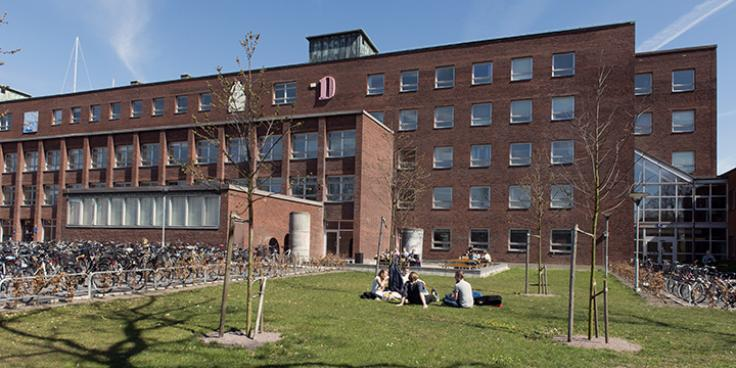
\includegraphics[height=0.41\textheight]{../img/ehuset}
\end{itemize}

Besök kurshemsidorna dagligen för mer information: 
\begin{itemize}
  \item \url{http://cs.lth.se/pgk} 
  \item \url{http://cs.lth.se/dod}
\end{itemize}
}

\end{document}
